\documentclass[a4,11pt]{aleph-notas}
% Actualizado en febrero de 2024
% Funciona con TeXLive 2022
% Para obtener solo el pdf, compilar con pdfLaTeX.
% Para obtener el xml compilar con XeLaTeX.

% -- Paquetes adicionales
\usepackage{aleph-moodle}
\moodleregisternewcommands
% Todos los comandos nuevos deben ir luego del comando anterior
\usepackage{aleph-comandos}
\usepackage{graphicx}
\usepackage{listings}
\usepackage{xcolor}
\usepackage{float}
\usepackage{amsmath} % Para ecuaciones
\usepackage{amssymb} % Para símbolos adicionales
\usepackage{tcolorbox} % Para crear la caja de fondo
\usepackage{lipsum}
\usepackage{booktabs}

\lstset{
  language=R,
  basicstyle=\ttfamily,
  keywordstyle=\color{blue},
  stringstyle=\color{orange},
  commentstyle=\color{gray},
  numbers=left,
  numberstyle=\tiny\color{gray},
  breaklines=true,
  frame=single,
  backgroundcolor=\color{lightgray!20}
}

% -- Datos
\institucion{Entrega Final -- Proyecto de Análisis Estadístico De Datos}
% \carrera{}
\asignatura{Proyecto de Análisis Estadístico De Datos}
\autor{Samuel Flores}
\logouno[3cm]{logo_ur.png}
\definecolor{colortext}{HTML}{DA0921}
\definecolor{colordef}{HTML}{00A1DE}
\fuente{montserrat}
% \fuente{mathpazo}

% -- Otros comandos
\newcommand{\nv}[1]{\textcolor{blue}{#1}}   % azul = modificado tras observaciones de la profesora
\newcommand{\apa}[1]{\par\hangindent=1.0cm\hangafter=1 #1\par}
\newcommand{\fuentefig}{\par{\footnotesize Fuente: elaboración propia con base en \texttt{bank\_data.csv}.}}

\begin{document}

\encabezado
\renewcommand{\tablename}{Tabla}
\renewcommand{\figurename}{Figura}
\linespread{1.15}\selectfont

%%%%%%%%%%%%%%%%%%%%%%%%%%%%%%%%%%%%%%%%
\begin{center}
\textbf{\large Compromiso y actividad de los clientes de un banco multinacional: ANOVA y modelos de regresión}
\end{center}

%%%%%%%%%%%%%%%%%%%%%%%%%%%%%%%%%%%%%%%%
\section*{1. Introducción}

\subsection*{1.1 Justificación y estado del arte}
La retención y el nivel de compromiso (\emph{engagement}) de los clientes son una preocupación estratégica del sector bancario: ante la competencia de entidades tradicionales y actores digitales, retener a un cliente resulta más rentable que adquirir uno nuevo (Kaur y Kaur, 2020). El conjunto \texttt{bank\_data.csv} reúne información demográfica, socioeconómica, de suscripción y de comportamiento de más de un millón de clientes de ocho ciudades, y permite un análisis completo, desde la calidad de los datos hasta la contrastación de hipótesis mediante ANOVA y regresión.

La literatura sobre deserción (\emph{churn}) bancaria es amplia. Kaur y Kaur (2020) compararon regresión logística, árboles de decisión, k-vecinos y bosques aleatorios. Singh et al. (2024) propusieron un flujo de preprocesamiento y comparación de modelos con una aplicación de visualización (RShiny) y sugirieron modelos localizados por país o región, pertinente con ocho ciudades. Li y Yan (2025) aplicaron balanceo de clases y valores SHAP, y hallaron que las variables transaccionales y de comportamiento pesan más que las demográficas; de ahí la hipótesis de este trabajo. La metodología sigue a Montgomery et al. (2021) en ANOVA y regresión lineal y a Hosmer et al. (2013) en regresión logística.

\section*{2. Planteamiento del problema y pregunta de investigación}
Los bancos recopilan grandes volúmenes de información de sus clientes, pero no siempre es evidente qué variables se asocian con que un cliente permanezca activo o comprometido; identificar esas asociaciones --o su ausencia-- es un paso previo a cualquier modelo de retención. La pregunta es:

\begin{quote}
\emph{¿Existe una asociación estadísticamente significativa entre las características demográficas (edad, género, ciudad) y de suscripción (nivel de suscripción) de los clientes bancarios y su nivel de compromiso (\texttt{Engagement\_Score}) y estado de actividad (\texttt{Is\_Active})?}
\end{quote}

Complementaria: ¿qué variables, de existir asociación, tienen mayor fuerza explicativa sobre la probabilidad de que un cliente se mantenga activo?

\section*{3. Objetivos}
\textbf{Objetivo general.} Analizar la relación entre las características demográficas, socioeconómicas y de suscripción de los clientes bancarios y su nivel de actividad y de compromiso, \nv{mediante ANOVA y modelos de regresión,} a partir de un conjunto de datos bancario multinacional.

\textbf{Objetivos específicos.}
\begin{itemize}
    \item Describir la estructura, la calidad y la distribución de las variables del conjunto de datos \texttt{bank\_data.csv}, e identificar y documentar sus problemas de calidad (faltantes, atípicos, inconsistencias).
    \item Explorar, mediante estadística descriptiva y análisis bivariado, las posibles asociaciones entre las variables demográficas y de suscripción y el estado de actividad y el compromiso de los clientes.
    \item \nv{Contrastar mediante ANOVA y regresión lineal múltiple el efecto de las variables explicativas sobre el compromiso (Objetivos 1 y 2 del análisis).}
    \item \nv{Evaluar mediante regresión logística la asociación de las variables con la actividad, verificando los supuestos de cada técnica (Objetivo 3 del análisis).}
\end{itemize}

%%%%%%%%%%%%%%%%%%%%%%%%%%%%%%%%%%%%%%%%
\section*{4. Marco metodológico}

\subsection*{4.1 Fuente, población y variables}
Los datos provienen del conjunto público \emph{Bank data} de Kaggle (sandippandey123, 2026): 1.000.050 registros (uno por cliente) y 8 variables. No se dispone de documentación sobre el diseño de muestreo; se trata como una muestra no probabilística y los resultados se interpretan sin pretensión de generalización. La Tabla~\ref{tab:variables} resume las variables; además de las 7 originales de análisis, se derivaron \texttt{Age\_Group}, \texttt{Salary\_Level}, \texttt{Engagement\_Level} (cualitativas ordinales) y \texttt{Engagement\_c} (truncada a [0, 100]).

\begin{table}[!htb]\centering\small\linespread{1}\selectfont
\caption{Descripción de las variables (* = variable derivada)}\label{tab:variables}
\begin{tabular}{llp{3.4cm}r}
\toprule
Variable & Descripción & Tipo (escala) & \% falt. \\
\midrule
ID & Identificador del cliente & Cualit. (nominal) & 0,0 \\
Gender & Male, Female, Non-Binary & Cualit. (nominal) & 0,0 \\
City & Ocho ciudades & Cualit. (nominal) & 10,0 \\
Subscription\_Tier & Basic, Premium, Pro & Cualit. (ordinal) & 0,0 \\
Is\_Active & Cliente activo (sí/no) & Cualit. (nominal) & 0,0 \\
Age\_Group* & 18-29, 30-44, 45-59, 60+ & Cualit. (ordinal) & 2,0 \\
Salary\_Level* & Cuatro tramos de salario & Cualit. (ordinal) & 5,0 \\
Engagement\_Level* & Bajo/Medio/Alto (media $\pm$ 1 DE) & Cualit. (ordinal) & 8,0 \\
Age & Edad en años (18--79) & Cuant. (razón) & 2,0 \\
Salary & Ingreso anual, USD & Cuant. (razón) & 5,0 \\
Engagement\_Score & Puntaje de compromiso & Cuant. (intervalo) & 8,0 \\
Engagement\_c* & Engagement truncado a [0, 100] & Cuant. (intervalo) & 8,0 \\
\bottomrule
\end{tabular}
\par\vspace{2pt}{\footnotesize Fuente: elaboración propia con base en \texttt{bank\_data.csv}.}
\end{table}

\subsection*{4.2 Calidad de los datos y preparación}
\textbf{Duplicados:} no hay identificadores repetidos (se conservó un registro por cliente). \textbf{Faltantes:} \texttt{Age} 2,0\%, \texttt{Salary} 5,0\%, \texttt{Engagement\_Score} 8,0\% y \texttt{City} 10,0\% (Tabla~\ref{tab:faltantes}); \texttt{Gender}, \texttt{Subscription\_Tier} e \texttt{Is\_Active} están completas. La prueba de independencia entre cada indicador de faltante y el estado de actividad no es significativa en ningún caso ($p\geq 0{,}435$), un indicio --no una prueba-- de que los faltantes no dependen de la respuesta. Los modelos usan los 771.145 clientes con información completa (77,1\%), y la sensibilidad se evalúa con imputación por la mediana. \textbf{Valores fuera de rango:} \texttt{Engagement\_Score} tiene 25 valores negativos (mínimo $-9{,}38$) y 3.549 superiores a 100 (máximo $132{,}41$). Con media 60,0 y desviación 15,0, una distribución normal produciría unos 3.582 valores fuera de [0, 100], cifra compatible con los 3.574 observados; se interpretan, por tanto, como colas de la distribución y no como errores de captura. Se conservó la variable original y se creó \texttt{Engagement\_c}, truncada, que se usa en los modelos.

\begin{table}[!htb]\centering\small\linespread{1}\selectfont
\caption{Valores faltantes por variable y asociación con el estado de actividad}\label{tab:faltantes}
\begin{tabular}{lrrr}
\toprule
Variable & Faltantes & Porcentaje & p (faltante vs. estado) \\
\midrule
Edad & 20.001 & 2,0\% & 0,606 \\
Salario & 50.002 & 5,0\% & 0,534 \\
Engagement Score & 80.004 & 8,0\% & 0,435 \\
Ciudad & 100.005 & 10,0\% & 0,825 \\
\bottomrule
\end{tabular}
\par\vspace{2pt}{\footnotesize Fuente: elaboración propia con base en \texttt{bank\_data.csv}.}
\end{table}


%%%%%%%%%%%%%%%%%%%%%%%%%%%%%%%%%%%%%%%%
\subsection*{4.3 Técnicas, hipótesis y supuestos}
La pregunta involucra una respuesta continua (\texttt{Engagement\_Score}) y una dicotómica (\texttt{Is\_Active}), explicadas por predictores mixtos, con una muestra muy grande. Se emplean: (i) \textbf{ANOVA} de uno y dos factores sobre el engagement (Objetivo 1); (ii) \textbf{regresión lineal múltiple}, técnica principal, equivalente a un ANOVA con covariables (Objetivo 2):
\[
\begin{split}
\text{Engagement}_i={}&\beta_0+\beta_1\,\text{Suscripción}_i+\beta_2\,\text{Edad}_i+\beta_3\,\text{Salario}_i\\
&+\beta_4\,\text{Género}_i+\beta_5\,\text{Ciudad}_i+\varepsilon_i,\quad \varepsilon_i\sim N(0,\sigma^2);
\end{split}
\]
y (iii) \textbf{regresión logística} para la actividad, con razones de odds ajustadas y el engagement como explicativa (Objetivo 3). Las covariables se reescalan (edad en décadas, salario en decenas de miles de USD, engagement en decenas de puntos) para que los coeficientes sean interpretables.

\textbf{Hipótesis (Entrega 1).} \textbf{H$_1$ (general):} el engagement y el nivel de suscripción están asociados con la probabilidad de que el cliente permanezca activo, mientras que las variables puramente demográficas (edad, género, ciudad) no presentan, por sí solas, asociación significativa. Su contraste formal usa \textbf{H$_0$:} ninguna variable explicativa se asocia con el estado de actividad, frente a \textbf{H$_1'$:} al menos una sí. En el ANOVA, $H_0:\mu_1=\dots=\mu_k$; en las regresiones, para cada término, $H_0:\beta_j=0$ (prueba $F$ marginal en el modelo lineal y razón de verosimilitud en el logístico). Se usa $\alpha=0{,}05$ con ajuste de Holm sobre los valores $p$ por término. El desempeño predictivo del modelo logístico se evalúa en una partición aleatoria 70/30 mediante el área bajo la curva ROC (AUC). Como verificación adicional, que la descripción pública de la base sugiere apta para aprendizaje automático, se ajustó un bosque aleatorio (Random Forest) capaz de capturar relaciones no lineales e interacciones. Los modelos describen asociaciones, no causalidad.

%%%%%%%%%%%%%%%%%%%%%%%%%%%%%%%%%%%%%%%%
\section*{5. Análisis descriptivo}

\subsection*{5.1 Variables cualitativas}
La Tabla~\ref{tab:freq} resume la composición de la base. El género y las ocho ciudades se reparten de forma prácticamente equitativa (33\% y 12,5\% cada categoría), la suscripción se concentra en el plan Basic (50,0\%) y el 69,9\% de los clientes está activo, de modo que ``Activo'' es la clase mayoritaria (Figura~\ref{fig:cuali}). La tasa de actividad es casi idéntica entre ciudades y planes (Figura~\ref{fig:cuali}, parte inferior): oscila entre 69,8\% y 70,2\%.

\begin{table}[!htb]\centering\small\linespread{1}\selectfont
\caption{Composición de las variables cualitativas (frecuencia relativa)}\label{tab:freq}
\begin{tabular}{lp{10.5cm}}
\toprule
Variable & Categorías (frecuencia relativa) \\
\midrule
Género & Female 33,3\%; Male 33,4\%; Non-Binary 33,3\% \\
Ciudad & Berlin 12,5\%; London 12,5\%; Mumbai 12,5\%; New York 12,5\%; Paris 12,5\%; Sydney 12,5\%; Tokyo 12,6\%; Toronto 12,4\% \\
Suscripción & Basic 50,0\%; Premium 30,0\%; Pro 19,9\% \\
Estado de actividad & Inactivo 30,1\%; Activo 69,9\% \\
Grupo de edad & 18-29 19,3\%; 30-44 24,2\%; 45-59 24,3\%; 60 o más 32,2\% \\
Nivel salarial & Hasta 60 mil 25,0\%; 60-90 mil 25,1\%; 90-120 mil 25,0\%; Más de 120 mil 25,0\% \\
Nivel de engagement & Bajo 15,9\%; Medio 68,0\%; Alto 16,0\% \\
\bottomrule
\end{tabular}
\par\vspace{2pt}{\footnotesize Fuente: elaboración propia con base en \texttt{bank\_data.csv}.}
\end{table}


\begin{figure}[!htb]\centering
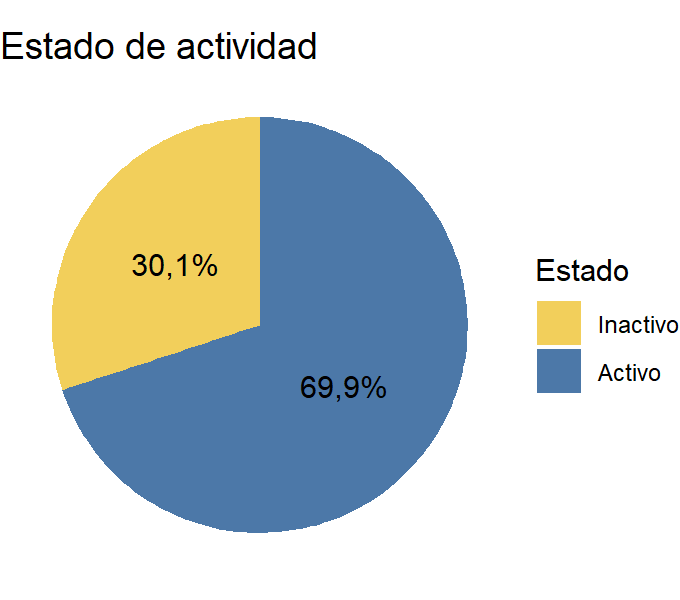
\includegraphics[width=.48\linewidth]{figs/fEstado.png}\hfill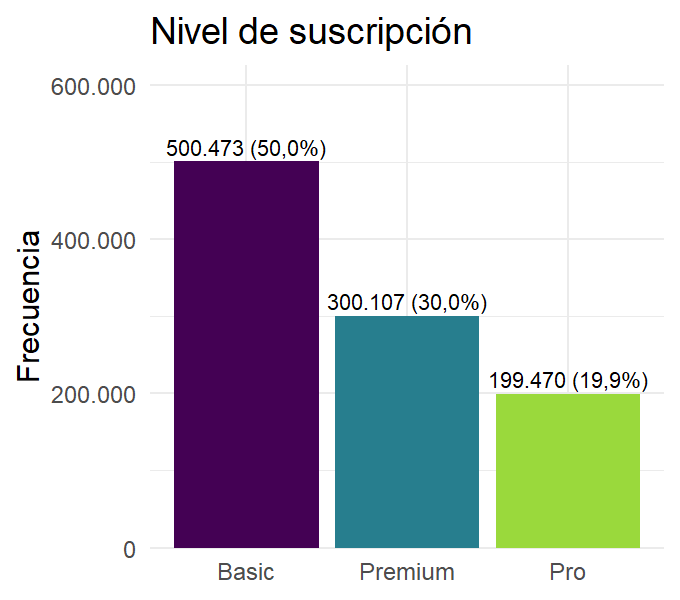
\includegraphics[width=.48\linewidth]{figs/fTier.png}\\[2pt]
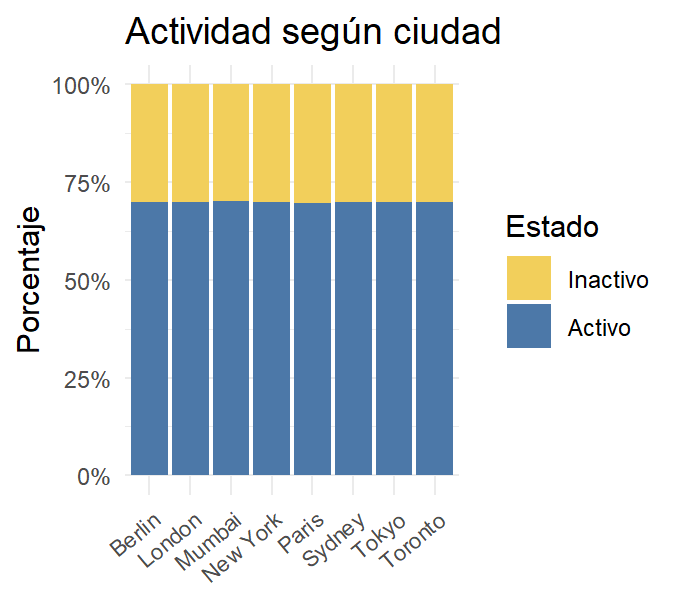
\includegraphics[width=.48\linewidth]{figs/fBivCity.png}\hfill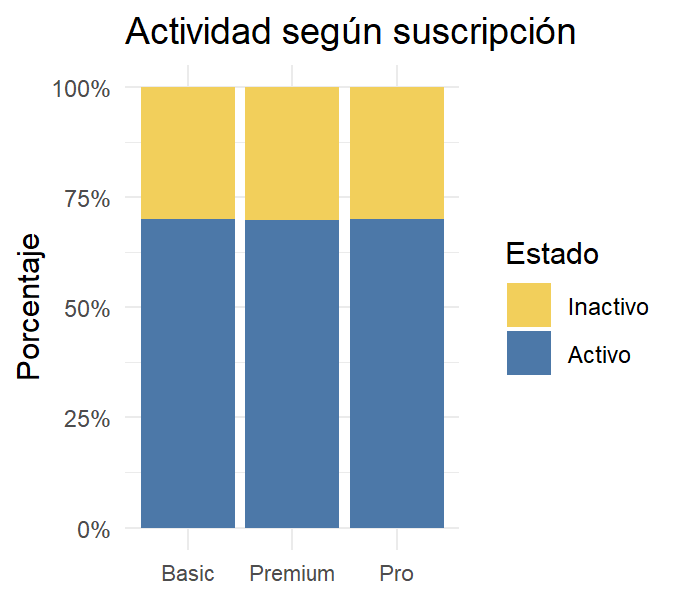
\includegraphics[width=.48\linewidth]{figs/fBivTier.png}
\caption{Estado de actividad, nivel de suscripción y estado de actividad según ciudad y suscripción}\label{fig:cuali}
\fuentefig
\end{figure}


\subsection*{5.2 Variables cuantitativas}
La edad (media 48,5; CV 36,9\%) y el salario (media 89.999 USD; CV 38,5\%) tienen asimetría nula y curtosis de 1,80, el valor teórico de una distribución uniforme (Tabla~\ref{tab:cuant}, Figura~\ref{fig:cuant}), una forma atípica para ingresos reales. El \emph{engagement} tiene forma de campana, con asimetría nula y curtosis 3,00, centrada en 60,0 con una dispersión relativa de 25,0\%.

\begin{table}[!htb]\centering\small\linespread{1}\selectfont
\caption{Estadígrafos de las variables cuantitativas (engagement sin truncar)}\label{tab:cuant}
\begin{tabular}{lrrr}
\toprule
Estadístico & Edad & Salario (USD) & Engagement \\
\midrule
n & 980.049 & 950.048 & 920.046 \\
Media & 48,49 & 89.999,46 & 60,00 \\
Mediana & 49,00 & 89.964,26 & 59,99 \\
Desviación estándar & 17,87 & 34.622,34 & 15,02 \\
Coef. de variación (\%) & 36,86 & 38,47 & 25,03 \\
Mínimo & 18,00 & 30.000,05 & -9,38 \\
Máximo & 79,00 & 149.999,73 & 132,41 \\
Coef. de asimetría & -0,00 & 0,00 & 0,00 \\
Curtosis (normal = 3) & 1,80 & 1,80 & 3,00 \\
\bottomrule
\end{tabular}
\par\vspace{2pt}{\footnotesize Fuente: elaboración propia con base en \texttt{bank\_data.csv}.}
\end{table}


\begin{figure}[!htb]\centering
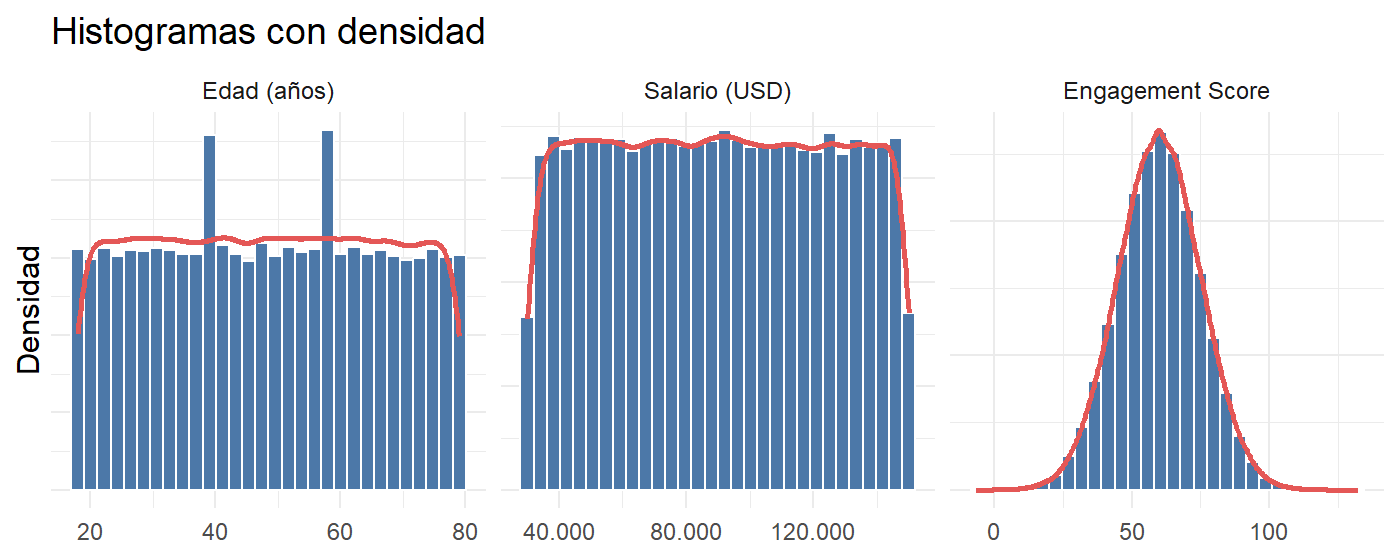
\includegraphics[width=.48\linewidth]{figs/fHist.png}\hfill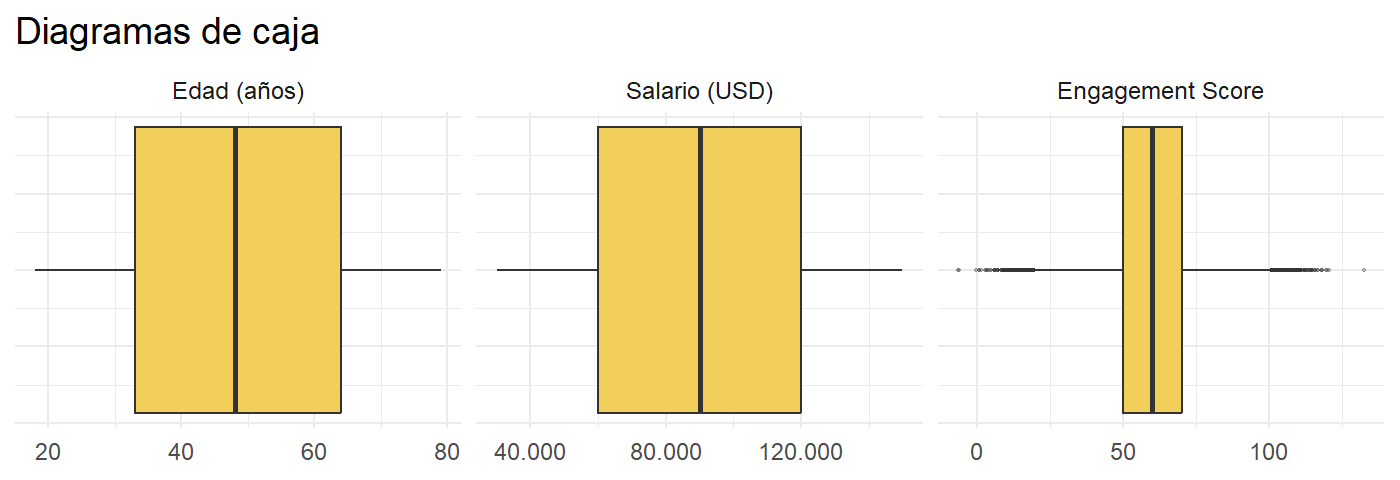
\includegraphics[width=.48\linewidth]{figs/fBox.png}
\caption{Histogramas con densidad y diagramas de caja de edad, salario y engagement}\label{fig:cuant}
\fuentefig
\end{figure}

\subsection*{5.3 Asociaciones bivariadas}
Ninguna de las 12 pruebas bivariadas es significativa tras el ajuste de Holm (Tablas~\ref{tab:chi} y~\ref{tab:ttest}). La V de Cramér máxima es 0,0029 (ciudad), un efecto despreciable; el mayor $|d|$ de Cohen entre activos e inactivos es 0,0042 (salario, $p=0{,}061$ sin ajustar; 0,727 con Holm), y el mayor $|r|$ entre variables cuantitativas es 0,0012 (edad y engagement). Las medias de engagement por suscripción, género y ciudad difieren como máximo 0,17 puntos. Con un millón de clientes, incluso diferencias mínimas podrían salir significativas; que no lo sean y que los tamaños de efecto sean prácticamente cero indica ausencia de relación, no falta de potencia (Figura~\ref{fig:biv}).

\begin{table}[!htb]\centering\small\linespread{1}\selectfont
\caption{Variables cualitativas y estado de actividad (chi-cuadrado de independencia)}\label{tab:chi}
\begin{tabular}{lrrrrrr}
\toprule
Variable & gl & Chi-cuadrado & p & p (Holm) & V de Cramér & \% activos (mín-máx) \\
\midrule
Género & 2 & 1,73 & 0,422 & 1,000 & 0,0013 & 69,9-70,0 \\
Ciudad & 7 & 7,75 & 0,355 & 1,000 & 0,0029 & 69,8-70,2 \\
Suscripción & 2 & 0,83 & 0,661 & 1,000 & 0,0009 & 69,9-70,0 \\
Grupo de edad & 3 & 0,97 & 0,809 & 1,000 & 0,0010 & 69,9-70,0 \\
Nivel salarial & 3 & 3,45 & 0,327 & 1,000 & 0,0019 & 69,8-70,0 \\
Nivel de engagement & 2 & 0,90 & 0,638 & 1,000 & 0,0010 & 69,9-70,0 \\
\bottomrule
\end{tabular}
\par\vspace{2pt}{\footnotesize Fuente: elaboración propia con base en \texttt{bank\_data.csv}.}
\end{table}

\begin{table}[!htb]\centering\small\linespread{1}\selectfont
\caption{Variables cuantitativas según estado de actividad (t de Welch)}\label{tab:ttest}
\begin{tabular}{lrrrrrr}
\toprule
Variable & Media inactivos & Media activos & Diferencia & d de Cohen & p & p (Holm) \\
\midrule
Edad & 48,48 & 48,50 & 0,02 & 0,0013 & 0,551 & 1,000 \\
Salario & 90.101,16 & 89.955,75 & -145,41 & -0,0042 & 0,061 & 0,727 \\
Engagement & 59,95 & 59,99 & 0,04 & 0,0024 & 0,288 & 1,000 \\
\bottomrule
\end{tabular}
\par\vspace{2pt}{\footnotesize Fuente: elaboración propia con base en \texttt{bank\_data.csv}.}
\end{table}


\begin{figure}[!htb]\centering
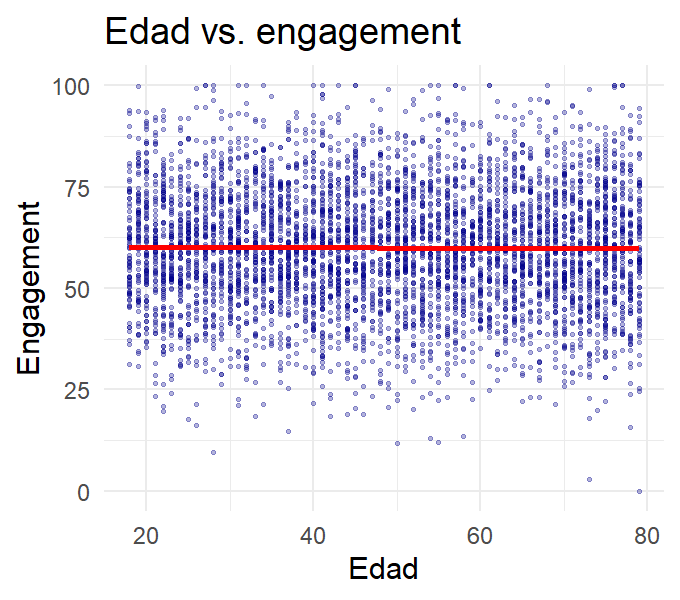
\includegraphics[width=.32\linewidth]{figs/fScatAgeEng.png}\hfill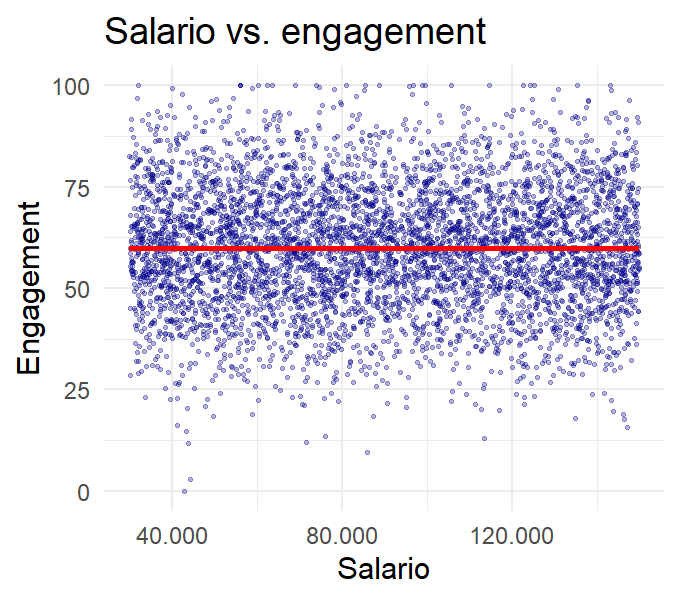
\includegraphics[width=.32\linewidth]{figs/fScatSalEng.png}\hfill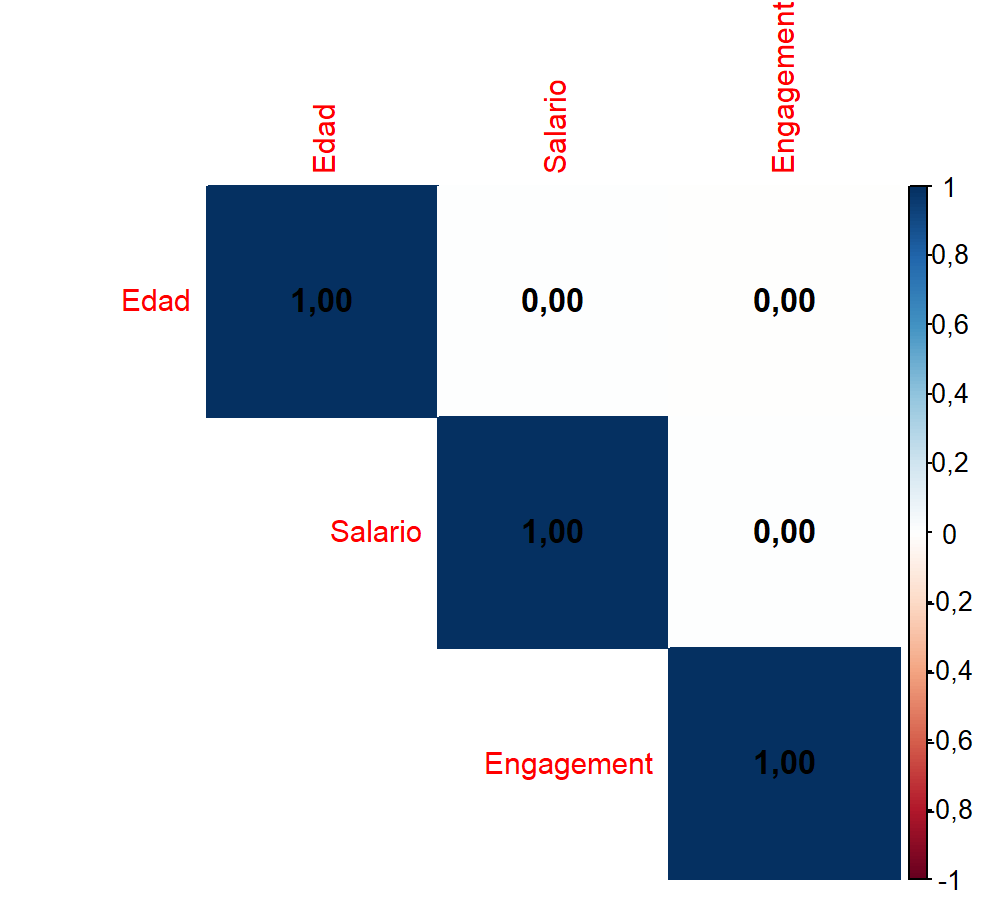
\includegraphics[width=.32\linewidth]{figs/fCorr.png}
\caption{Dispersión edad--engagement y salario--engagement (muestra de 5.000 clientes) y matriz de correlación}\label{fig:biv}
\fuentefig
\end{figure}

\subsection*{5.4 Bondad de ajuste}
Género, ciudad y cada valor de la edad son compatibles con categorías equiprobables ($p=0{,}708$; $0{,}587$ y $0{,}617$), consistente con datos generados de forma uniforme. El engagement se ajusta de cerca a la curva normal (asimetría nula y curtosis 3,00; Figura~\ref{fig:cuant}).



%%%%%%%%%%%%%%%%%%%%%%%%%%%%%%%%%%%%%%%%
\section*{6. Verificación de supuestos}
La Tabla~\ref{tab:sup} resume la verificación. La normalidad de los residuos del ANOVA y del modelo lineal se rechaza con Shapiro-Wilk ($p=0{,}006$ y $0{,}032$, sobre 5.000 residuos); con tantas observaciones la prueba detecta desviaciones mínimas, y los gráficos de residuos (Figura~\ref{fig:diag}) muestran un ajuste cercano a la normal, por lo que la inferencia es razonable por el teorema central del límite. Los demás supuestos se cumplen: varianzas homogéneas (Levene $p=0{,}452$; Bartlett $p=0{,}367$), homocedasticidad (Breusch-Pagan $p=0{,}331$), independencia de errores (Durbin-Watson $=2{,}003$), especificación (RESET $p=0{,}294$), ausencia de multicolinealidad (GVIF ajustado máx. $=1{,}000$), 16.554 eventos por parámetro en la logística, linealidad del logit ($p=0{,}872$) y ausencia de observaciones influyentes (Cook máx. $=0{,}00009$). Breusch-Pagan, Durbin-Watson, RESET e influencia se calcularon sobre submuestras de 50.000 registros por costo computacional.

\begin{table}[!htb]\centering\small\linespread{1}\selectfont
\caption{Verificación de supuestos de las técnicas empleadas}\label{tab:sup}
\begin{tabular}{lp{3.3cm}p{5.6cm}l}
\toprule
Modelo & Supuesto & Evidencia & Conclusión \\
\midrule
ANOVA & Normalidad de residuos & Shapiro-Wilk (n = 5.000): p = 0,006 & No se cumple \\
ANOVA & Homogeneidad de varianzas & Levene p = 0,452; Bartlett p = 0,367 & Se cumple \\
ANOVA & Independencia & Un registro por cliente (ID único) & Se asume por diseño \\
Lineal & Normalidad de residuos & Shapiro-Wilk (n = 5.000): p = 0,032 & No se cumple \\
Lineal & Homocedasticidad & Breusch-Pagan: p = 0,331 & Se cumple \\
Lineal & Independencia de errores & Durbin-Watson = 2,003 (p = 0,704) & Se cumple \\
Lineal & Linealidad / especificación & RESET: p = 0,294 & Se cumple \\
Lineal & Ausencia de multicolinealidad & GVIF ajustado máx. = 1,000 (umbral 2,24) & Se cumple \\
Logístico & Eventos por parámetro & Eventos por parámetro = 16.554 (regla: 10) & Se cumple \\
Logístico & Ausencia de multicolinealidad & GVIF ajustado máx. = 1,000 (umbral 2,24) & Se cumple \\
Logístico & Linealidad del logit & RV términos cuadráticos: p = 0,872 & Se cumple \\
Logístico & Observaciones influyentes & Cook máx. = 0,00009 & Se cumple \\
\bottomrule
\end{tabular}
\par\vspace{2pt}{\footnotesize Fuente: elaboración propia con base en \texttt{bank\_data.csv}.}
\end{table}


%%%%%%%%%%%%%%%%%%%%%%%%%%%%%%%%%%%%%%%%
\section*{7. Aplicación e interpretación}

\subsection*{7.1 Objetivo 1: ANOVA del engagement}
Ningún factor presenta diferencias significativas en el engagement medio tras el ajuste de Holm (Tabla~\ref{tab:aov}); la más cercana es el género ($F=2{,}949$; $p=0{,}052$ sin ajustar, 0,262 con Holm). El mayor eta cuadrado es 0,000009 (ciudad), un efecto despreciable. Para el plan de suscripción, Tukey indica diferencias de hasta 0,023 puntos (p ajustado mínimo $=0{,}866$), y el ANOVA de dos factores no halla interacción suscripción por género ($p=0{,}244$; Figura~\ref{fig:aov}, cuyo eje vertical abarca menos de 0,2 puntos). Decisión: no se rechaza H$_0$ en ningún factor.

\begin{table}[!htb]\centering\small\linespread{1}\selectfont
\caption{ANOVA de un factor sobre el engagement (truncado)}\label{tab:aov}
\begin{tabular}{lrrrrr}
\toprule
Factor & gl & F & p & p (Holm) & Eta cuadrado \\
\midrule
Suscripción & 2; 920.043 & 0,512 & 0,599 & 1,000 & 0,000001 \\
Género & 2; 920.043 & 2,949 & 0,052 & 0,262 & 0,000006 \\
Ciudad & 7; 828.154 & 1,080 & 0,373 & 1,000 & 0,000009 \\
Grupo de edad & 3; 901.655 & 1,107 & 0,345 & 1,000 & 0,000004 \\
Nivel salarial & 3; 874.135 & 0,884 & 0,449 & 1,000 & 0,000003 \\
\bottomrule
\end{tabular}
\par\vspace{2pt}{\footnotesize Fuente: elaboración propia con base en \texttt{bank\_data.csv}.}
\end{table}


\begin{figure}[!htb]\centering
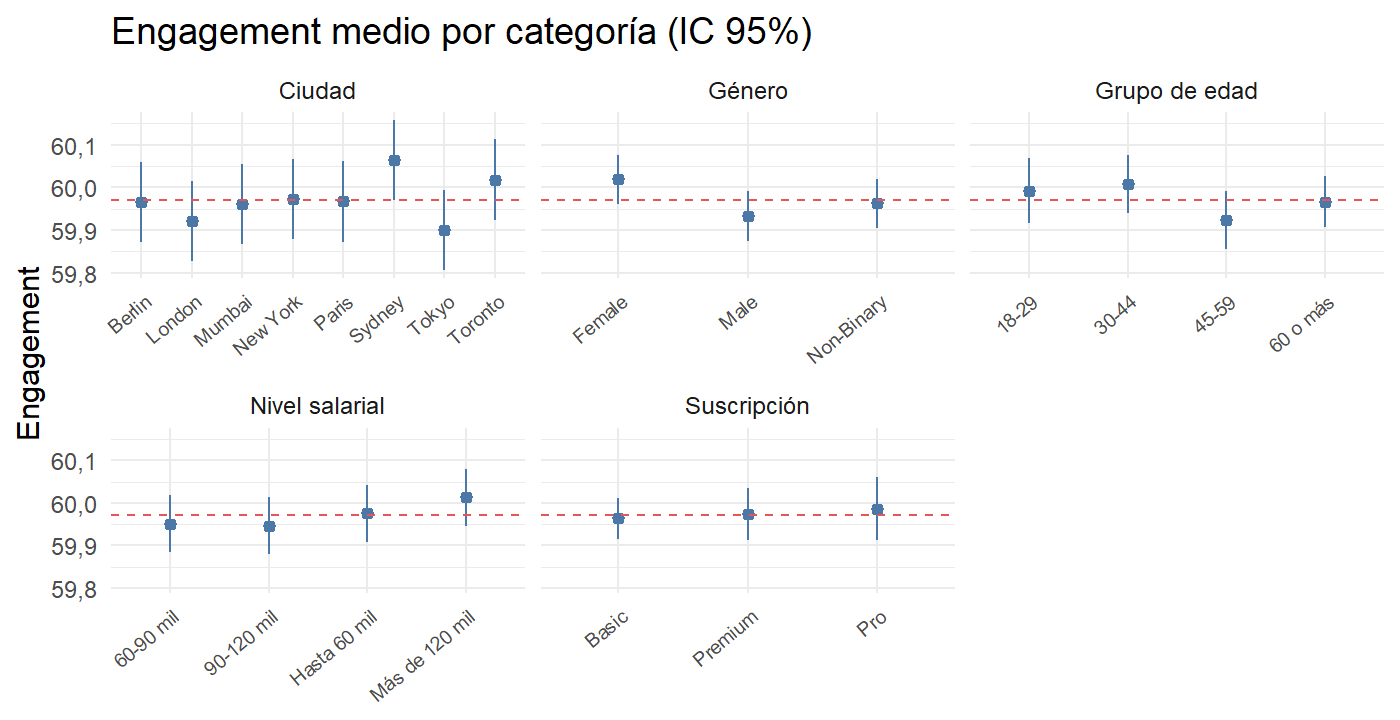
\includegraphics[width=.48\linewidth]{figs/fAovMedias.png}\hfill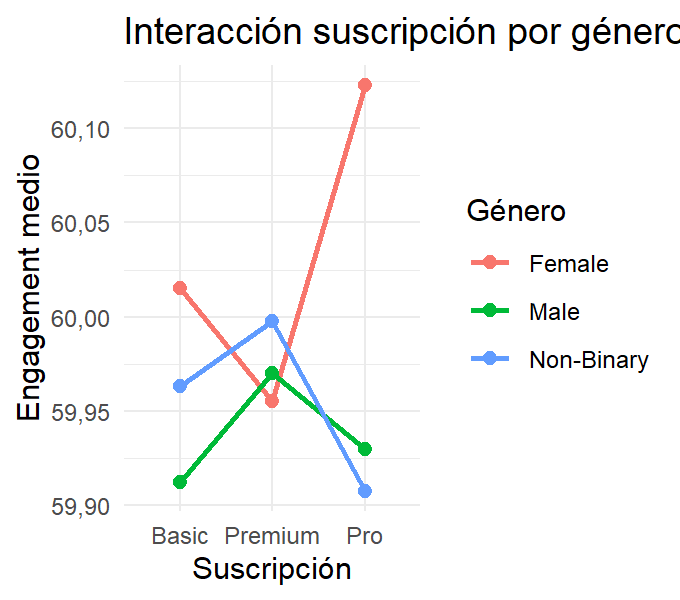
\includegraphics[width=.48\linewidth]{figs/fInter.png}
\caption{Engagement medio por categoría (IC 95\%) e interacción suscripción por género}\label{fig:aov}
\fuentefig
\end{figure}

\subsection*{7.2 Objetivo 2: regresión lineal múltiple}
Con ajuste de Holm, ninguna variable se asocia de forma significativa con el engagement (Tabla~\ref{tab:lmanova}); el mayor eta cuadrado parcial es 0,000010 (ciudad), despreciable, y el modelo explica menos de 0,01\% de la variabilidad. Cada década adicional de edad se asocia con un cambio de $-0{,}009$ puntos de engagement (IC 95\%: $-0{,}028$ a $0{,}010$), manteniendo lo demás constante. Los coeficientes de suscripción (Premium $+0{,}011$; Pro $+0{,}023$) y salario ($+0{,}003$ por 10.000 USD) son igualmente despreciables. Un coeficiente aislado, \texttt{Género: Male} ($-0{,}086$; $p=0{,}040$), no sobrevive al contraste global del género ($p=0{,}113$; $p_{\text{Holm}}=0{,}566$), por lo que se considera efecto del azar entre múltiples comparaciones. Los coeficientes estandarizados son $-0{,}00105$ (edad) y $0{,}00062$ (salario).

\begin{table}[!htb]\centering\small\linespread{1}\selectfont
\caption{Tabla ANOVA del modelo lineal (tipo II)}\label{tab:lmanova}
\begin{tabular}{lrrrrr}
\toprule
Término & gl & F & p & p (Holm) & Eta cuadrado parcial \\
\midrule
Suscripción & 2 & 0,136 & 0,873 & 1,000 & 0,000000 \\
Edad & 1 & 0,848 & 0,357 & 1,000 & 0,000001 \\
Salario & 1 & 0,295 & 0,587 & 1,000 & 0,000000 \\
Género & 2 & 2,179 & 0,113 & 0,566 & 0,000006 \\
Ciudad & 7 & 1,140 & 0,334 & 1,000 & 0,000010 \\
\bottomrule
\end{tabular}
\par\vspace{2pt}{\footnotesize Fuente: elaboración propia con base en \texttt{bank\_data.csv}.}
\end{table}


\begin{figure}[!htb]\centering
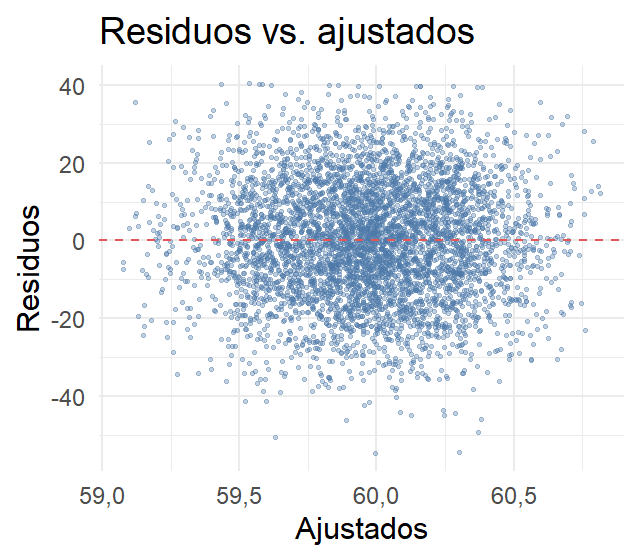
\includegraphics[width=.32\linewidth]{figs/fDiagRes.png}\hfill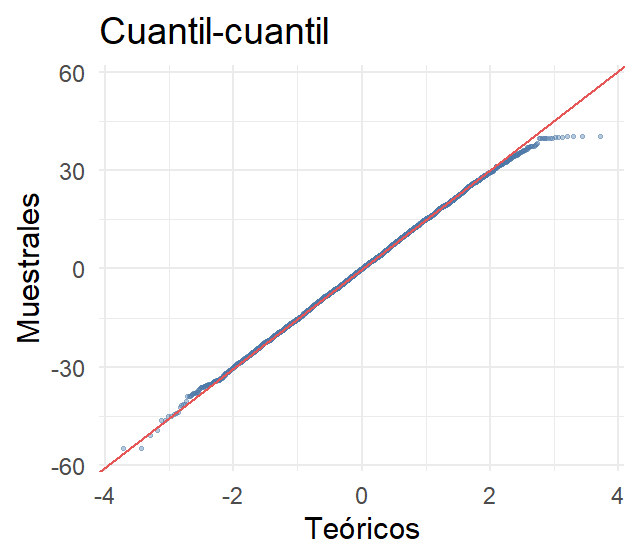
\includegraphics[width=.32\linewidth]{figs/fDiagQQ.png}\hfill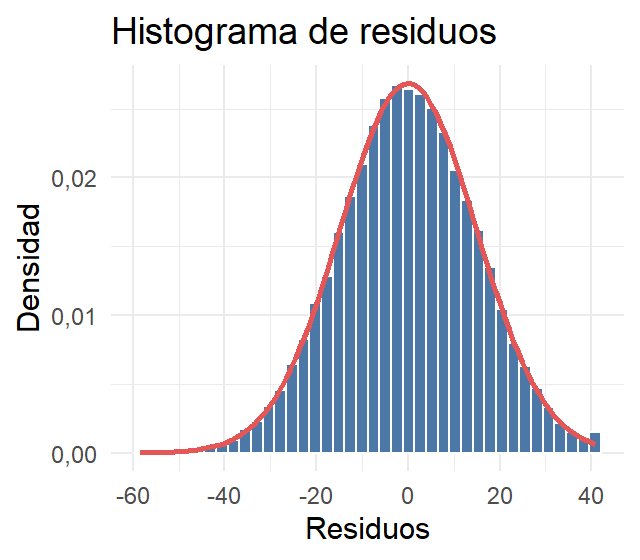
\includegraphics[width=.32\linewidth]{figs/fDiagHist.png}
\caption{Diagnóstico de residuos del modelo lineal (muestra de 5.000 residuos)}\label{fig:diag}
\fuentefig
\end{figure}

\subsection*{7.3 Objetivo 3: regresión logística del estado de actividad}
El modelo completo no mejora de forma estadísticamente significativa al modelo nulo ($\chi^2=15{,}90$, gl $=14$, $p=0{,}320$) y su ajuste es mínimo (pseudo-$R^2$ de McFadden $=0{,}00002$; de Nagelkerke $=0{,}00003$). Con Holm, ninguna variable es significativa (Tabla~\ref{tab:lrt}); el salario es la más cercana ($p=0{,}046$ sin ajustar; 0,276 con Holm; OR $=0{,}9986$ por cada 10.000 USD, IC 95\%: 0,9972 a 1,0000). Por cada 10 puntos adicionales de engagement, los odds de estar activo se multiplican por 1,002 (IC 95\%: 0,999 a 1,005; $p=0{,}245$; Tabla~\ref{tab:or}), es decir, no cambian. En la muestra de prueba el AUC es 0,501, una capacidad discriminativa prácticamente nula (Figura~\ref{fig:roc}); con el umbral igual a la prevalencia de entrenamiento, la exactitud es 49,4\% (sensibilidad 48,4\%, especificidad 51,6\%) frente a 69,9\% de predecir siempre ``Activo'' (matriz de confusión: 35.920 y 78.283 aciertos sobre 231.344 clientes de prueba). La calibración por deciles muestra probabilidades predichas de aproximadamente 69,6\% a 70,3\%, casi sin variación. \textbf{Sensibilidad:} el odds ratio del engagement es 1,002 en el modelo base, sin truncar el puntaje y con imputación de faltantes ($n=1.000.050$), de modo que las conclusiones no dependen del tratamiento de atípicos ni de faltantes.

\begin{table}[!htb]\centering\small\linespread{1}\selectfont
\caption{Pruebas de razón de verosimilitud por término (modelo logístico)}\label{tab:lrt}
\begin{tabular}{lrrrr}
\toprule
Término & gl & Chi-cuadrado (RV) & p & p (Holm) \\
\midrule
Engagement Score & 1 & 1,35 & 0,245 & 1,000 \\
Suscripción & 2 & 0,25 & 0,883 & 1,000 \\
Edad & 1 & 0,01 & 0,941 & 1,000 \\
Salario & 1 & 3,98 & 0,046 & 0,276 \\
Género & 2 & 2,78 & 0,250 & 1,000 \\
Ciudad & 7 & 7,55 & 0,374 & 1,000 \\
\bottomrule
\end{tabular}
\par\vspace{2pt}{\footnotesize Fuente: elaboración propia con base en \texttt{bank\_data.csv}.}
\end{table}

\begin{table}[!htb]\centering\small\linespread{1}\selectfont
\caption{Razones de odds de estar activo (ciudad omitida)}\label{tab:or}
\begin{tabular}{lrrr}
\toprule
Término & Odds ratio & IC 95\% & p \\
\midrule
Engagement (+10 puntos) & 1,0019 & [0,9987; 1,0052] & 0,245 \\
Suscripción: Premium & 0,9990 & [0,9878; 1,0103] & 0,862 \\
Suscripción: Pro & 1,0025 & [0,9897; 1,0155] & 0,701 \\
Edad (+10 años) & 1,0001 & [0,9974; 1,0028] & 0,941 \\
Salario (+10.000 USD) & 0,9986 & [0,9972; 1,0000] & 0,046 \\
Género: Male & 0,9901 & [0,9784; 1,0020] & 0,104 \\
Género: Non-Binary & 0,9969 & [0,9851; 1,0089] & 0,612 \\
\bottomrule
\end{tabular}
\par\vspace{2pt}{\footnotesize Fuente: elaboración propia con base en \texttt{bank\_data.csv}.}
\end{table}


\begin{figure}[!htb]\centering
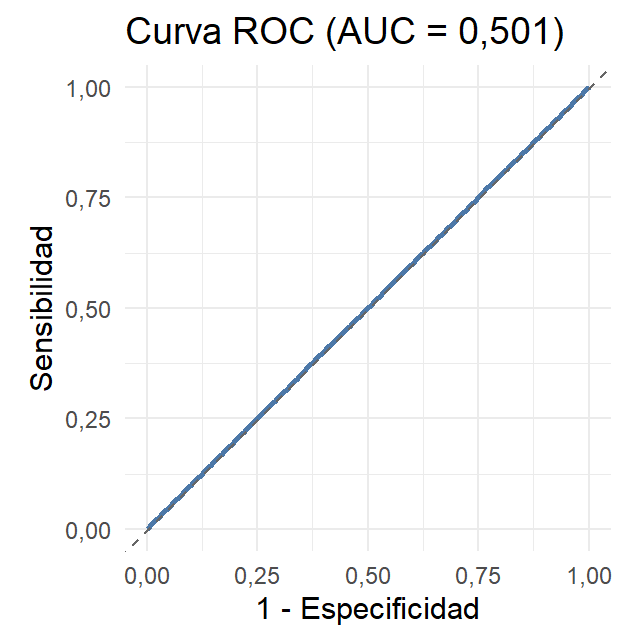
\includegraphics[width=.48\linewidth]{figs/fROC.png}\hfill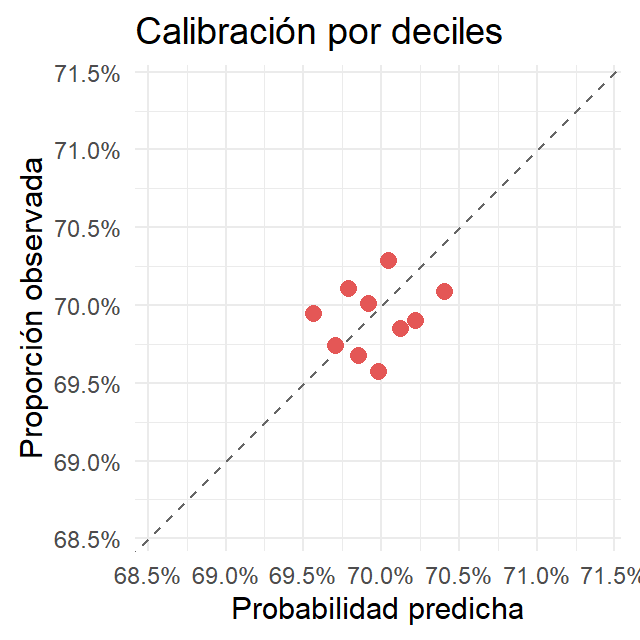
\includegraphics[width=.48\linewidth]{figs/fCal.png}
\caption{Curva ROC y calibración por deciles en la muestra de prueba}\label{fig:roc}
\fuentefig
\end{figure}

\subsection*{7.4 Verificación con un modelo no lineal}
La logística solo captura relaciones lineales y aditivas, por lo que se ajustó un bosque aleatorio (200 árboles; submuestra aleatoria de 100.000 clientes con información completa; partición 70/30) con las seis variables explicativas. El AUC en la muestra de prueba fue 0,4996, indistinguible del azar y coherente con el 0,501 de la regresión logística. Las importancias de Gini más altas corresponden a salario y engagement (6.455 y 6.392), seguidas de edad (3.811), ciudad (1.358), género (708) y suscripción (676); esas diferencias reflejan que las variables continuas ofrecen más puntos de corte posibles, y no un poder predictivo real, pues el modelo no predice mejor que el azar. Un modelo no lineal tampoco encuentra información en estas variables, lo que refuerza que el límite está en los datos y no en la técnica.

%%%%%%%%%%%%%%%%%%%%%%%%%%%%%%%%%%%%%%%%
\section*{8. Discusión}
\textbf{Hipótesis.} Ninguna variable explicativa resultó significativa tras el ajuste de Holm, por lo que no se rechaza H$_0$ y no se respalda la hipótesis general H$_1$ de la Entrega 1, que esperaba asociación del engagement y la suscripción con la actividad. La ausencia de asociación es, en sí misma, un hallazgo. \textbf{Frente a la literatura.} A diferencia de Li y Yan (2025), donde las variables de comportamiento superaron a las demográficas, aquí ni siquiera el engagement se asocia con la actividad. La capacidad discriminativa nula (AUC $=0{,}501$ en la logística y $0{,}4996$ en un bosque aleatorio) contrasta con los modelos de Kaur y Kaur (2020) y Li y Yan (2025), que emplean variables transaccionales ausentes en esta base. Una explicación adicional es la naturaleza de los datos: distribuciones uniformes de edad y salario, correlaciones cercanas a cero, 69,9\% de actividad en todos los grupos y un engagement casi perfectamente normal son compatibles con datos simulados de forma independiente, donde no cabe esperar relaciones. \textbf{Modelos por ciudad.} Respecto de la sugerencia de Singh et al. (2024), la ciudad no mostró efecto, por lo que estos datos no aportan evidencia a favor de modelos localizados.

\section*{9. Conclusiones}
\begin{enumerate}
    \item Ni las características demográficas (edad, género, ciudad), ni el salario, ni el nivel de suscripción se asocian de forma significativa con el engagement ni con la actividad (ANOVA, regresión lineal y logística con ajuste de Holm).
    \item Los tamaños de efecto son despreciables: eta cuadrado máximo 0,000010, V de Cramér máxima 0,0029 y $|d|$ máximo 0,0042; el modelo lineal explica menos de 0,01\% de la variabilidad del engagement.
    \item El modelo logístico no discrimina mejor que el azar (AUC $=0{,}501$) y no supera a predecir siempre ``Activo'' (49,4\% frente a 69,9\% de exactitud); un bosque aleatorio tampoco (AUC $=0{,}4996$), por lo que el límite está en la información de la base y no en la técnica.
    \item No se respalda la hipótesis general H$_1$ de la Entrega 1: el engagement no modifica los odds de actividad (OR $=1{,}002$ por 10 puntos).
    \item Los resultados son robustos al tratamiento de los datos (truncamiento del engagement e imputación) y los supuestos principales se cumplen, salvo la normalidad estricta de los residuos, esperable con tantas observaciones.
    \item El patrón es compatible con una base simulada; antes de usarla para decisiones de negocio debe validarse con datos reales y variables transaccionales.
\end{enumerate}

\section*{10. Limitaciones}
(i) Fuente secundaria sin documentación de muestreo y con comportamiento compatible con datos simulados; (ii) solo tres variables cuantitativas y cuatro cualitativas originales, sin variables transaccionales ni definición explícita de deserción (la guía pide seis y seis; se compensa en parte con variables derivadas); (iii) los modelos usan 77,1\% de los registros por los faltantes; (iv) con más de un millón de clientes las pruebas formales rechazan efectos triviales, por lo que se reportan tamaños de efecto; (v) diseño transversal: solo asociaciones; (vi) los modelos suponen aditividad y linealidad, y los diagnósticos se calcularon sobre submuestras.

\section*{11. Recomendaciones}
Incorporar variables transaccionales y temporales (frecuencia y monto de movimientos, productos, antigüedad) y definir con precisión la deserción; validar con datos reales y documentados del banco; explorar modelos no lineales con interacciones (árboles, bosques aleatorios) y modelos por ciudad, como sugieren Singh et al. (2024); y usar validación cruzada y remuestreo para evaluar la estabilidad de los resultados.

%%%%%%%%%%%%%%%%%%%%%%%%%%%%%%%%%%%%%%%%
\section*{Bibliografía}
\apa{Hosmer, D. W., Lemeshow, S., \& Sturdivant, R. X. (2013). \emph{Applied logistic regression} (3.ª ed.). John Wiley \& Sons.}
\apa{Kaur, I., \& Kaur, J. (2020). Customer churn analysis and prediction in banking industry using machine learning. En \emph{2020 Sixth International Conference on Parallel, Distributed and Grid Computing (PDGC)} (pp. 434--437). IEEE. \url{https://doi.org/10.1109/PDGC50313.2020.9315761}}
\apa{Li, Y., \& Yan, K. (2025). Prediction of bank credit customers churn based on machine learning and interpretability analysis. \emph{Data Science in Finance and Economics}, 5(1), 19--34. \url{https://doi.org/10.3934/DSFE.2025002}}
\apa{Montgomery, D. C., Peck, E. A., \& Vining, G. G. (2021). \emph{Introduction to linear regression analysis} (6.ª ed.). John Wiley \& Sons.}
\apa{R Core Team. (2026). \emph{R: A language and environment for statistical computing}. R Foundation for Statistical Computing. \url{https://www.R-project.org/}}
\apa{sandippandey123. (2026). \emph{Bank data} [Conjunto de datos]. Kaggle. \url{https://www.kaggle.com/datasets/sandippandey123/bank-data}}
\apa{Singh, P. P., Anik, F. I., Senapati, R., Sinha, A., Sakib, N., \& Hossain, E. (2024). Investigating customer churn in banking: A machine learning approach and visualization app for data science and management. \emph{Data Science and Management}, 7(1), 7--16. \url{https://doi.org/10.1016/j.dsm.2023.09.002}}

\section*{Declaración de uso de IA}
Se utilizó una herramienta de inteligencia artificial generativa (Claude, de Anthropic) como apoyo para estructurar y depurar el código en R y mejorar la redacción del documento. \nv{[Confirmar y ajustar:]} la interpretación de los resultados, la verificación de los supuestos y las conclusiones fueron revisadas, comprendidas y asumidas por el grupo, y todo el código fue ejecutado y comprendido por sus integrantes.

\section*{Participación del equipo}
\begin{tabular}{p{5.2cm}p{9.5cm}}
\toprule
Integrante & Contribución \\
\midrule
Samuel Flores & \nv{[Describir aportes en cada etapa: datos, análisis, redacción, póster]} \\
\nv{[Integrante 2]} & \nv{[Describir aportes]} \\
\bottomrule
\end{tabular}

\end{document}
